\tocchapter{Aurrekarien analisia}

\section{Sarrera}
Gaur egun badaude ASS formatuko azpitituluak editatzeko aplikazioak, gehienak Microsoft-en Windows sistema eragilerako eta batzuk Linux-erako. Mac OS X sistemarako ordea, ez dago erabilgarria den aplikaziorik.
\section{Azpititulu editoreak}
Atal honetan denboran zehar erabiliak izan diren azpititulu editoreak aztertu eta konparatuko ditugu.
\subsection{Sub Station Alpha}
Programa honek hasi zuen gure proiektuaren inguruko dena, programarekin batera, SSA formatua sortu zelako (honetatik atera zen gaur erabiltzen den ASS formatua). Microsoft Windows-erako doainiko programa pribatiboa da, 1996. urtean sortua britaniar baten eskutik, \textit{Kotus} ezizenarekin ezagutua. Ateratako azken bertsioa 2000. urtekoa da, beraz honen garapena duela asko bertan behera utzi zen.

Garatzailearen esanetan, programaren funtzioa azpitituluak modu erraz batean eta kalitate handiarekin sortzea zen, garaiko garestiak eta motelak ziren tresna komertzialen ordezko bat sortzea hain zuzen ere.

Nahiz eta bere garapena gaur egun kantzelatua egon, oraindik jende askok erabiltzen du, programa sinplea delako eta beraz oso erreza erabiltzeko, baita bere garaian erabiltzen zutenen ohituragatik.

Hiru fitxategirekin lan egiten du:
\begin{itemize}
\item SSA script-a.
\item Bideo fitxategi bat.
\item Audio fitxategi bat.
\end{itemize}

Azpitituluak editatzeko, SSA fitxategia da behar dugun bakarra, baina azpitituluak sinkronizatzeko audio fitxategia kargatu behar dugu. Fitxategi honen formatua \textit{PCM WAV} motakoa izan behar da, 8 bitekoa eta kanal bakarrekoa (\textit{mono}). Bideoaren erabilera erreferentzia bat edukitzeko mugatzen da, azpitituluak ez dituelako erakusten prozesatu ondoren ikusiko diren bezala.
\begin{figure}[htb]
\begin{center}
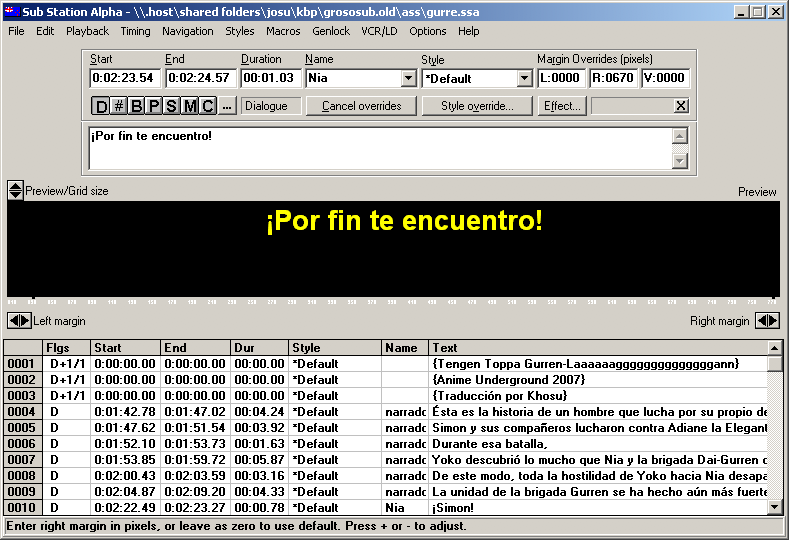
\includegraphics[width=\columnwidth, natwidth=789pt, natheight=540pt]{Pictures/Chapter2/ssa-script.png}
\caption{Sub Station Alpha azpititulu fitxategi batekin}
\label{ssa-script}
\end{center}
\end{figure}

\ref{ssa-script}~Irudian ikusten dugun bezala programak informazioa guztia lehio berdinean erakusten du. Nahiz eta erabilgarria izan, oso astuna suertatzen da beste programekin konparatuz. Honez gain, ezer arrarorik egin gabe, \textit{bug} askorekin topatuko gara lanean gabiltzan bitartean.

Aldaketak ez dira azpiko taulan egiten, goiko partean baizik, non aukeratua dugun lerroaren informazioa guztia eskuragarri dugun.

Aurrebista ez da batere zehatza, aukeratutako lerroa erakusten du bere letra-mota eta kolorearekin atzekalde beltzean soilik. Beraz, ez digu erakusten adibidez itzalaren kolorea, azpitituluaren posizioa pantailan, etab. Ikusten dugunez, aurrebista honek ez du funtzionalitate handirik.
\begin{figure}[htb]
\begin{center}
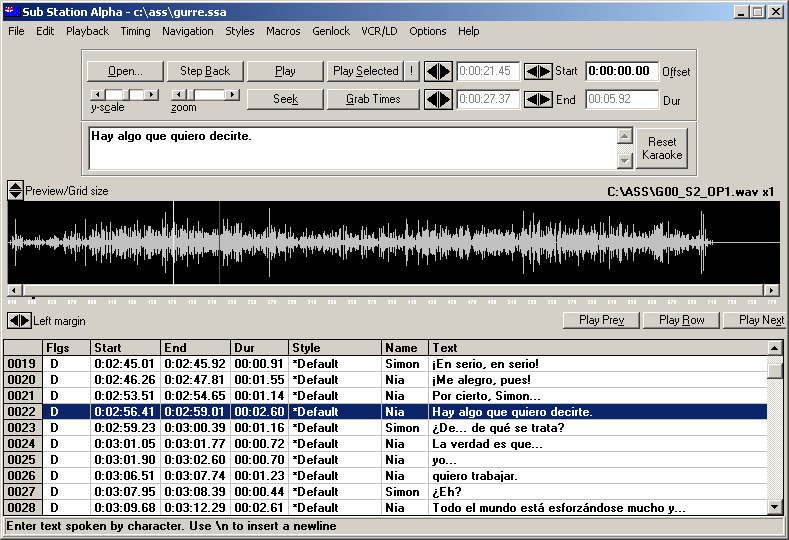
\includegraphics[width=\columnwidth, natwidth=789pt, natheight=540pt]{Pictures/Chapter2/ssa-audio.png}
\caption{Sub Station Alpha audio fitxategi batekin}
\label{ssa-audio}
\end{center}
\end{figure}

Azpitituluez gain audio fitxategi bat kargatzerakoan, \ref{ssa-audio}~Irudian ikusten dugunarekin topatuko gara. Azpitituluen aurrebistaren ordez, audioaren uhin-forma erakusten digu. Lerro baten hasiera eta bukaera denborak esleituko ditugu hemen saguaren bidez click eginez nahi dugun lekuan. Lehen aipatu dugun bezala, audioaren formatua ezin daiteke edozein izan, \textit{PCM WAV} formatuan egon behar da, 8 bitekoa eta kanal bakarrekoa, beraz ez da oso ondo entzuten MP3 edo OGG Vorbis-ekin alderatuz.

Ondorio bezala, Sub Station Alpha erabilgarria da, baina gaur egungo berriagoak diren aukerak erabiltzea gomendagarria da, erosoagoak direlako.

\subsection{Medusa}
2002. urtean, \textit{Sub Station Alpha}-ren garapena 2 urtez geldirik egon ondoren, editore hau kaleratu zuen programatzaile italiar batek, \textit{Kaidousama} ezizenarekin ezagutua. Urte honetarako, SSA formatuaren eboluzioa atera zen, \textit{Advanced Substation Alpha} (ASS), gaur egun erabiltzen dena hain zuzen. Aurreko programa bezala, hau baita Microsoft-en Windows sistema eragilerako garatu zen Visual Basic 6 erabiliz.

Aldaketa handiak suposatu zituen editore honek, gehienbat ASS formatuaren inplementazioagatik. Hauek dira aipagarrienak:
\begin{itemize}
\item ASS formatuaren erabilera natiboa.
\item Audio formatu gehiago erabili ditzake, adibidez \textit{MP3} edo \textit{OGG Vorbis}.
\item Bideo bidezko sinkronizazioa.
\item Sintaxiaren nabarmendua denbora errealean hau hobeto ulertzeko.
\item Karaokeak silaba bidez sinkonizatzeko aukera, azkarra eta erosoa.
\end{itemize}

Hala ere, lan egiteko modua bere aintzindariaren antzekoa da, horregatik lortu zuen \textit{Sub Station Alpha} erabiltzen zuten askok hau erabiltzea.
\begin{figure}[htb]
\begin{center}
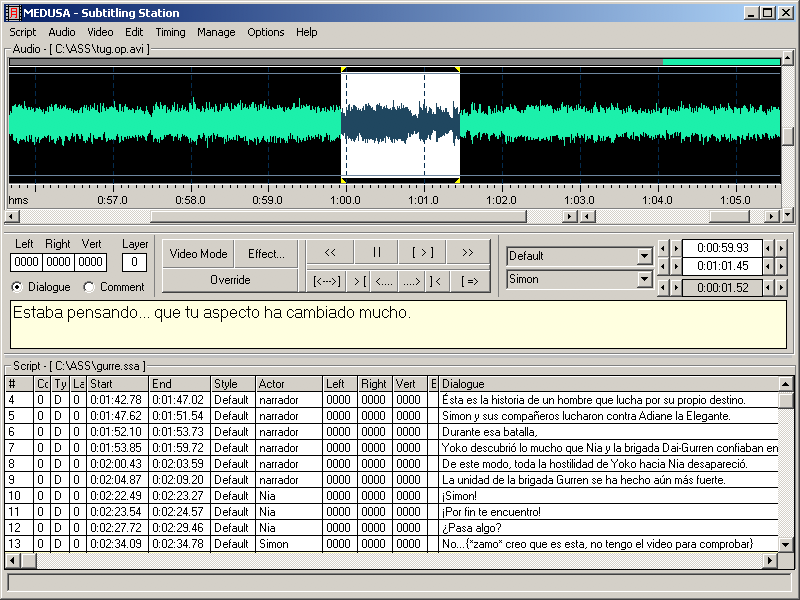
\includegraphics[width=\columnwidth, natwidth=800pt, natheight=600pt]{Pictures/Chapter2/medusa-audio.png}
\caption{Medusa editorea azpititulu eta audio fitxategi batekin}
\label{medusa-audio}
\end{center}
\end{figure}

\ref{medusa-audio}~Irudian ikusten dugunez, nahiz eta antzeko interfazea izan, askoz atseginagoagoa da bisualki, baita bere erabileran ere.

Funtzionalitate berriak sartu zituen, adibidez, aukeratutako audio zatia erreproduzitzeaz gain, honen testuingurua (aurreko eta ondorengo 500 milisegunduak), aukeratutakoaren hasiera, amaiera, etab. Honez gain, ASS formatuarekin lan egiten duenez, estilo mota berriak onartzen ditu. Azpitituluen aurrebista ere badu, VSFilter erabiliz.
\begin{figure}[htb]
\begin{center}
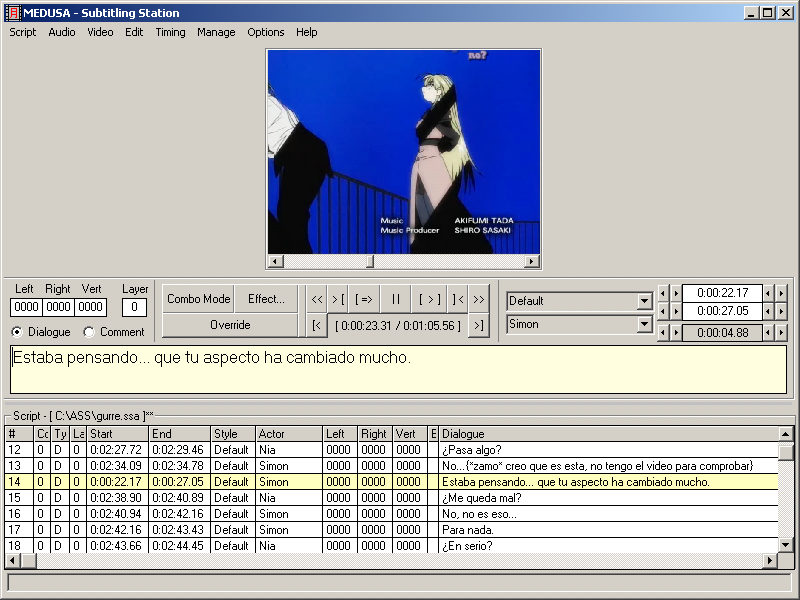
\includegraphics[width=\columnwidth, natwidth=800pt, natheight=600pt]{Pictures/Chapter2/medusa-bideo.png}
\caption{Medusa editorea azpititulu eta bideo fitxategi batekin}
\label{medusa-bideo}
\end{center}
\end{figure}

Bideo fitxategi bat kargatzerakoan, \ref{medusa-bideo}~Irudian ikusten dugunarekin aurkituko gara. Azpitituluak sinkronizatzeko erabili dezakegu hau, baita hauek ikusteko ere. Dena den, alde txar bat dauka: \textit{DirectShow} erabiltzen du, beraz erakusten dituen \textit{frame}-ak ez dira zehaztasun handiarekin benetakoak. Ondorioz, bideoaren frame batean jarritako azpititulu bat, probabilitate handiarekin beste frame batean agertuko da gero bideoan. Ikusten dugunez, nahiz eta \textit{Sub Station Alpha}-rekin konparatuz bideoarekin hobeto lan egin daitekeen, ez da oso erabilgarria.

\textit{Medusa}-k momentuan ekarri zuen funtzionalitate hoberena karaokeak sinkronizatzeko interfazea izan zen, \ref{medusa-karaoke}~Irudian ikusten duguna hain zuzen.
\begin{figure}[htb]
\begin{center}
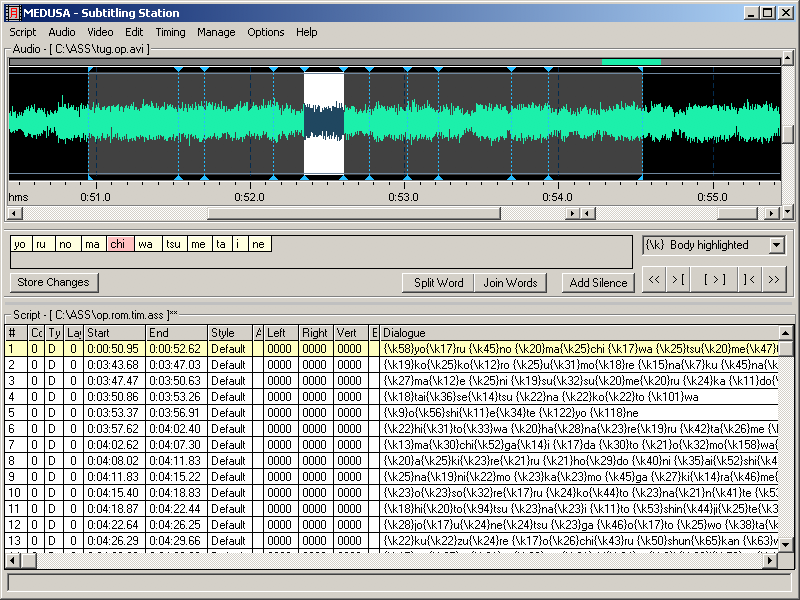
\includegraphics[width=\columnwidth, natwidth=800pt, natheight=600pt]{Pictures/Chapter2/medusa-karaoke.png}
\caption{Medusa editorearen karaokeak sinkronizatzeko interfazea}
\label{medusa-karaoke}
\end{center}
\end{figure}

Ikusten dugunez, silabaka banatzen da lerroko testua, eta hauek batu edo banatu eta isiluneak gehitu ahal ditzakegu. Gainera, silaba baten hasiera edo bukaera denbora aldatzean, bere ondokoak ere aldatzen dira (adibidez amaiera denbora murriztean, hurrengo silabaren hasiera denbora lehenago izango da). \textit{Sub Station Alpha}-rekin alderatuz, izugarrizko aurrerapena zen, honetan eskuz egin behar zirelako inolako laguntzarik gabe. Minutu t'erdiko abestiaren karaokea egitea \textit{Sub Station Alpha}-rekin ordu pare bateko esfortzua eskatzen zuen, \textit{Medusa}-rekin karaoke bera egitea 30 minutu inguru, hau da, laurden bat.

Ondorioz, nahiz eta bere aurrerakira baino programa hobeagoa izan, zenbait akats ditu. Adibidez, nahiz eta MP3-rekin lan egin ahal izan, hau kargatzerakoan PCM formatura pasatzen du, 16 bitekoa, \textit{estereo} eta 44 KHz-tako maiztasunarekin, eta disko gogorrean gordetzen du. 24 minutuko MP3 batek gutxi gora behera 30 MB-eko tamaina du, baina PCM-ra pasatzerakoan 300 MB-eko fitxategi bat lortuko dugu.

2004. urtean bere garapena bertan behera utzi zen, egileak Delphi-n birprogramatzea erabaki zuelako (\textit{ChronoSub} izenarekin), baina ez da berririk egon honen inguruan.

\subsection{Aegisub}
Hau da gaur egungo ASS formatuko azpititulu editorerik hoberena. Azpititulatzaile komunitateak berak garatu du, \textit{Sub Station Alpha}-k eta \textit{Medusa}-k zituzten arazoak konpontzeko asmoarekin.

Hasieran \textit{Visual SSA} izenarekin ezagutu zen, ondoren \textit{Visual ASS} bezala eta azkenik \textit{Aegisub} izenarekin geratu da. 2005. urtean agertu zen v1.00 \textit{beta} bertsioa, eta 1.07 bertsiotik aurrera bere kodea askatu zuten BSD\footnote{\url{http://en.wikipedia.org/wiki/BSD_license}} lizentzia batekin. Bere denbora librea azpititulatzen pasatzen zuten bi programatzailek hasi zuten proiektua, baina gaur egun jende asko dago garapen taldean, horregatik gaur egun dagoen aplikaziorik erabilena eta konpletuena da.

C++ lengoiaz garatuta dago, eta nahiz eta hasieran Windows-erako bakarrik izan, gaur egun Linux-en funtzionatzen du, baita Mac OS X-en ere (garatzaileen esanetan, baina honen inguruan aurrerago hitz egingo dugu).

Hauek dira programak dituen ezaugarri nagusiak:
\begin{itemize}
\item ASS formatuaren erabilera natiboa, honez gain SSA, SRT eta TXT formatuak inportatu ditzake.
\item Unicode testu kodifikazioan dauden fitxategiak erabil ditzake (oso erabilgarria beste hizkuntzetako karaktereak sartzeko).
\item Karaokeak modu automatizatuan egiteko aukera \textit{Lua} programazio lengoaia erabiliz.
\item Sintaxiaren nabarmendua.
\item Bideoak ireki ditzake \textit{AviSynth} erabiliz.
\item Azpitituluak erakusten ditu \textit{VSFilter} erabiliz, beraz prozesatu ondoren ikusiko diren bezala.
\item \textit{DirectShow}-k dekodifikatu dezakeen edozein audio fitxategirekin lan egiteko ahalmena.
\item Karaokeen sinkronizazioarako sistema aurreratua.
\item Itzulpen prozesurako laguntzaile bat.
\item Estiloak gorde daitezke script desberdinetan erabili ahal izateko.
\item Estiloak aplikatzeko laguntzailea bat.
\item Azpitituluen arteko kolisioak antzematen ditu.
\item Makroen erabilera zenbait ataza egiteko.
\item Azpitituluak modu grafikoan editatzeko aukera.
\end{itemize}

Bere atzean dagoen garapen taldeari esker, funtzionalitate asko eta onak ditu programa honek.

\begin{figure}[htbp]
\begin{center}
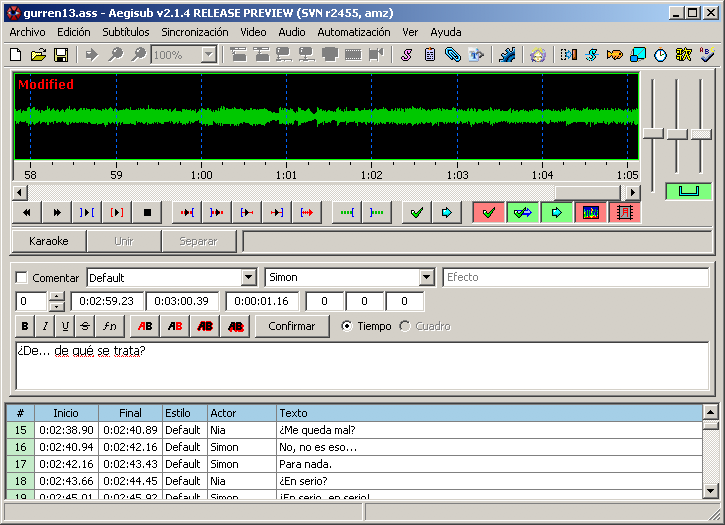
\includegraphics[width=\columnwidth, natwidth=725pt, natheight=525pt]{Pictures/Chapter2/aegisub-audio.png}
\caption{Aegisub editorea azpititulu eta audio fitxategi batekin}
\label{aegisub-audio}
\end{center}
\end{figure}

\ref{aegisub-audio}~Irudian ikus dezakegunez, interfazea antzekoa da \textit{Sub Station Alpha} eta \textit{Medusa}-rekin konparatuz, baina hauek baino erosoagoa da lan egiteko orduan, dauzkan aukera mordoagatik.

Audio bidezko sinkronizazioarako, erabili nahi ditugun teklak definitu ditzakegu, horrela aurreko bi programetan bezala lan egin ahal izateko. Audioa oso azkar kargatzen da programan eta ez ditu alde baterako fitxategi handiak erabiltzen. Honen ordez, ahal duen guztia kargatzen du RAM memorian modu azkar batean atzitu ahal izateko. Uhin-forma marrazteko funtzioa baita ere azkarra da, eta hau asko eskertzen dan sinkronizatzerakoan, asko mugitzen garela uhin-formaren ikuspegitik zehar. Honez gain, uhin-espektroa marraztu dezake \textit{FFT}\footnote{\url{http://en.wikipedia.org/wiki/Fast_Fourier_transform}} erabiliz. Hau oso erabilgarria da espektroan gizakion ahotsa modu errazean ikus dezakegulako.

Bideoa kargatzeaz eta ikusteaz gain, bere gainean lan egin dezakegu. Testua mugitu, biratu (hiru ardatzekiko), tamainaz aldatu, \textit{clip}-ak egin, etab. saguarekin modu erraz eta ikusgarri batean. Guzti hau ikusi dezakegu \ref{aegisub-bideo}~Irudian (ezkerraldean daude testuan aldaketak egiteko tresnak).

\begin{figure}[htbp]
\begin{center}
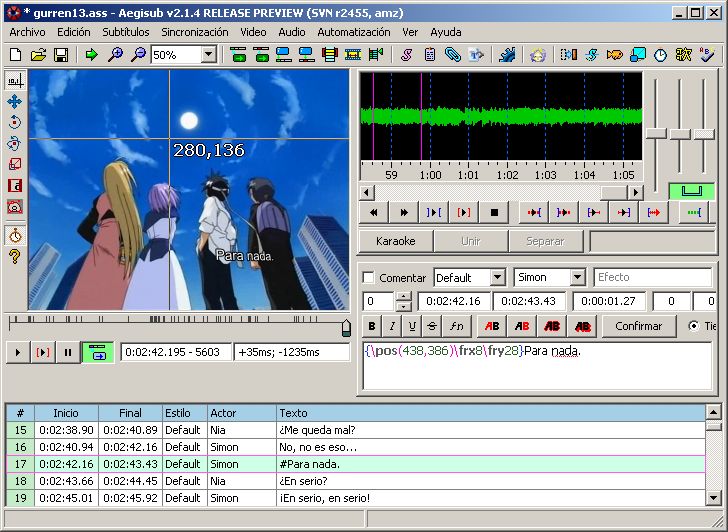
\includegraphics[width=\columnwidth, natwidth=728pt, natheight=532pt]{Pictures/Chapter2/aegisub-bideo.png}
\caption{Aegisub editorea azpititulu eta bideo fitxategi batekin}
\label{aegisub-bideo}
\end{center}
\end{figure}

Bestalde, post-prozesaketa aukerak eskeintzen ditu lehenengo aldiz mota honetako programetan, oso erabilgarriak diren ekintzak egin ahal izateko. Adibidez, tarte batean hurbil dauden azpitituluak modu jarraian ipiniko ditu, horrela azpitituluak momentu batez ez desagertuz, edo lerro bat bestearen gainean ez egoteko momentu batez. Beste adibide bat: azpitituluen denborak \textit{keyframe}\footnote{\url{http://en.wikipedia.org/wiki/Key_frame}} batetik hurbil badaude, honetara egokituko ditu. Guzti honetarako \ref{aegisub-post}~Irudian dagoen lehioa erabitzen da.

\begin{figure}[htbp]
\begin{center}
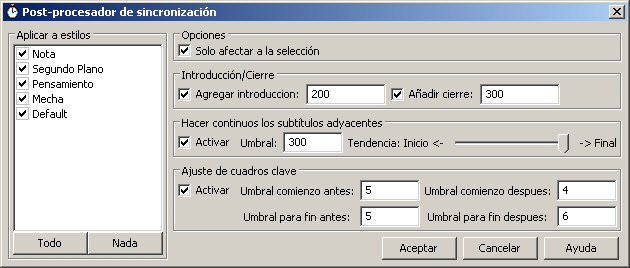
\includegraphics[width=\columnwidth, natwidth=630pt, natheight=268pt]{Pictures/Chapter2/aegisub-post.png}
\caption{Aegisub editorearen post-prozesaketa aukerak}
\label{aegisub-post}
\end{center}
\end{figure}

\begin{figure}[htp]
\begin{center}
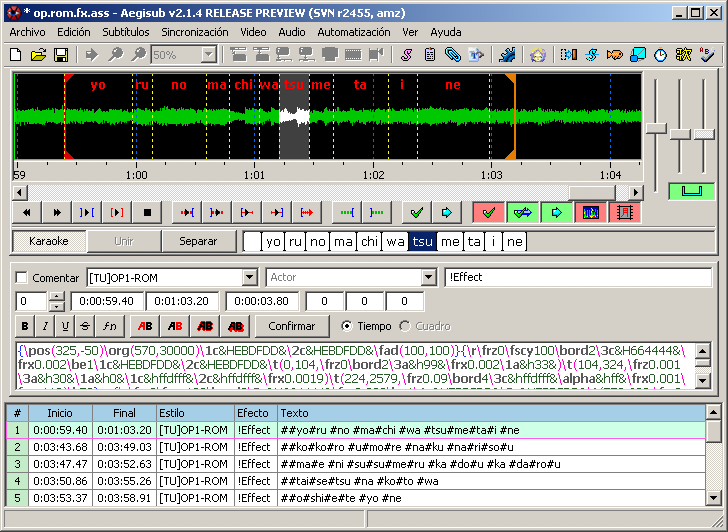
\includegraphics[width=\columnwidth, natwidth=728pt, natheight=532pt]{Pictures/Chapter2/aegisub-karaoke.png}
\caption{Aegisub editorearen karaokeak sinkronizatzeko interfazea}
\label{aegisub-karaoke}
\end{center}
\end{figure}

Azkenik, karaokeak egiteko \textit{Medusa}-k daukan sistemaren antzeko bat dauka \ref{aegisub-karaoke}~Irudian ikus dezakegun bezala, oso erosoa eta azkarra lan neketsu hau egiteko.

Honez gain, karaokeen gainean efektuak, aplika ditzakegu karaoke konplexuago eta politagoak egin ahal izateko, \textit{Lua}\footnote{\url{http://www.lua.org/}} \textit{scripting} lengoaiaren bidez. Hau existitu baino lehenago, kalkulu guztiak kalkulagailu bidez egiten ziren, lan oso neketsua eta motela izanik. Gainera, sortzen ditugun efektuak momentuan ikus ditzakegu horrela lan fluxua azkartuz.

Aurreko guztia kontuan hartuz, ondoriozta dezakegu hau dela gaur egun dagoen azpititulu editorerik hoberena eskeintzun duen guztiagatik eta kalitateagatik. Lehen esan bezala, suposatzen da Mac OS X-en funtzionatzen duela, eta horrela da, konpilatu eta exekuta dezakegu, baina guztiz apurtuta dago, adibidez, audio fitxategi bat kargatzerakoan erroreak agertuko zaizkigu eta ezingo dugu audioarekin lan egin.

\section{Konparaketa}
\ref{konparaketa}~taulan daude hiru programa hauen ezaugarriak. Bertan ikus dezakegunez, Aegisub da hiruretatik hoberena.
\begin{longtable}{|l|c|c|c|}
\hline
& \grey Sub Station Alpha & \grey Medusa & \grey Aegisub\\
\hline
\endhead
\hline
\caption{\label{konparaketa}Aztertutako programen ezaugarriak}
\endfoot
\grey Bertsioa & 4.08 & 0.1.2.0 & 2.00alpha\\
\hline
\grey Garapena & \red Bertan behera & \red Bertan behera & \green Aktiboa\\
\hline
\grey Lizentzia & \red Itxia & \red Itxia & \green BSD\\
\hline
\grey Lengoaia & Visual Basic & Visual Basic & C++\\
\hline
\multicolumn{4}{|l|}{\bgrey \textbf{Azpititulu formatuak}}\\
\hline
\grey SSA & \green Bai(natiboa) & \green Bai & \green Bai\\
\hline
\grey ASS & \red Ez & \green Bai(natiboa) & \green Bai(natiboa)\\
\hline
\grey SRT & \red Ez & \green Bai & \green Bai\\
\hline
\grey Testu planoa & \green Bai & \green Bai & \green Bai\\
\hline
\multicolumn{4}{|l|}{\bgrey \textbf{Karaktere kodifikazioa}}\\
\hline
\grey Lokala & \green Bai(natiboa) & \green Bai(natiboa) & \green Bai\\
\hline
\grey Unicode & \red Ez & \red Ez & \green Bai(natiboa)\\
\hline
\grey Autodetekzioa & \red Ez & \red Ez & \green Bai\\
\hline
\multicolumn{4}{|l|}{\bgrey \textbf{Sistema eragileak}}\\
\hline
\grey Microsoft Windows & \green Bai & \green Bai & \green Bai\\
\hline
\grey Linux & \red Ez & \red Ez & \yellow Osatugabea\\
\hline
\grey Mac OS X & \red Ez & \red Ez & \red Erabilezina\\
\hline
\multicolumn{4}{|l|}{\bgrey \textbf{Audioa}}\\
\hline
\grey PCM WAV & \yellow 8 bit mono & \green Bai & \green Bai\\
\hline
\grey MP3 & \red Ez & \green Bai & \green Bai\\
\hline
\grey Ogg Vorbis & \red Ez & \green Bai & \green Bai\\
\hline
\grey AAC & \red Ez & \red Ez & \green Bai\\
\hline
\grey AC3 & \red Ez & \red Ez & \green Bai\\
\hline
\grey Bideotik & \green Bai & \red Ez & \green Bai\\
\hline
\grey Uhin-forma & \green Bai & \green Bai & \green Bai\\
\hline
\grey Espektroa & \red Ez & \red Ez & \green Bai\\
\hline
\multicolumn{4}{|l|}{\bgrey \textbf{\textit{Typesetting}}}\\
\hline
\grey Bisualki & \red Ez & \red Ez & \green Bai\\
\hline
\grey Estilo editorea & \green Bai & \green Bai & \green Bai\\
\hline
\grey Estilo kudeatzailea & \green Bai & \green Bai & \green Bai\\
\hline
\grey Estilo aurrebista & \green Bai & \red Ez & \green Bai\\
\hline
\multicolumn{4}{|l|}{\bgrey \textbf{Audio sinkronizazioa}}\\
\hline
\grey Elkarrizketak & \green Bai & \green Bai & \green Bai\\
\hline
\grey Karaokeak & \yellow Sinplea & \green Bai & \green Bai\\
\hline
\multicolumn{4}{|l|}{\bgrey \textbf{Azpitituluen gaineko eragiketak}}\\
\hline
\grey Shift, Split eta Join & \green Bai & \green Bai & \green Bai\\
\hline
\grey Bikoiztu & \red Ez & \red Ez & \green Bai\\
\hline
\grey Undo/Redo & \red Ez & \red Ez & \green Bai\\
\hline
\grey Sintaxi nabarmendua & \red Ez & \green Bai & \green Bai\\
\hline
\grey Regex & \red Ez & \red Ez & \green Bai\\
\hline
\multicolumn{4}{|l|}{\bgrey \textbf{Tresnak}}\\
\hline
\grey Itzulpen laguntzailea & \red Ez & \red Ez & \green Bai\\
\hline
\grey Zuzentzailea & \green Bai & \red Ez & \green Bai\\
\hline
\grey Karaoke efektuak & \red Ez & \yellow Sinplea & \green Bai\\
\hline
\multicolumn{4}{|l|}{\bgrey \textbf{Bestelakoak}}\\
\hline
\grey Automatikoki gorde & \green Bai & \red Ez & \green Bai\\
\hline
\grey Segurtasun kopiak & \red Ez & \red Ez & \green Bai\\
\hline
\grey Dokumentu anitz & \red Ez & \red Ez & \red Ez\\
\end{longtable}

\section{Ondorioak}

Kapitulu honetan aztertu dugunez, aplikazio bat dago azpititulugintzako lehengo postuan, \textit{Aegisub} hain zuzen ere. Nahiz eta garatzaileen esanetan Mac OS X-en funtzionatu, ez da batere erabilgarria. Konpilatu eta exekutatu dezakegu, baina adibidez ezin dugu audiorik kargatu eta honekin lan egin, beraz, programaren funtzionalitatea asko murrizten da.

\textit{Aegisub}-ek lizentzia irekia du, BSD lizentzia hain zuzen ere, beraz, zergatik ez hau eraldatu eta guri interesatzen zaigun plataformarako egokitu? Alde batetik, askoz zailagoa da aplikazioa konpontzea berri bat hastea baino, gauza gutxik funtzionatzen dutelako, bakarrik ASS formatuaren kudeaketa eta honen gaineko eragiketak. Bestalde, \textit{Aegisub} C++ lengoaian dago idatzita eta wxWidgets\footnote{\url{http://www.wxwidgets.org/}}-ekin dago programatuta. Honen ondorioz, programa ez dago sisteman integratua, ez dauka beste aplikazio guztien itxura berdina.
Mac OS X-eko aplikazioa natiboak ordez, Objective-C\footnote{\url{http://en.wikipedia.org/wiki/Objective-C}} lengoaian daude idatzita. Objektuei zuzendutako lengoaia da, C lengoaiaren gainean eraikia, honi Smalltalk\footnote{\url{http://en.wikipedia.org/wiki/Smalltalk}}-eko mezuak gehituz. Aplikazio grafikoak egiteko, Cocoa\footnote{\url{http://developer.apple.com/cocoa/}} API-a erabiltzen da.

Dena den, \textit{Aegisub}-ek funtzionalitate asko dauzka, eta proiektu honetan, garapen denbora kontuan edukita ezin izango dugu hain programa konplexua egin, beraz funtzionalitate bakar batzuk inplementatuko dira. Adibidez audioa eta bideoarekin ez du lanik egingo programak, honen inplementazioa gure mugetatik guztiz ateratzen delako.
